% !TEX TS-program = XeLaTeX
% use the following command: 
% all document files must be coded in UTF-8
\documentclass{textolivre}
% for anonymous submission
%\documentclass[anonymous]{textolivre}
% to create HTML use 
%\documentclass{textolivre-html}
% See more information on the repository: https://github.com/leolca/textolivre

% Metadata
\begin{filecontents*}[overwrite]{article.xmpdata}
    \Title{Ensino remoto e ressignificação de práticas e papéis na educação}
    \Author{Joyce Fettermann \sep Annabell Dell Real Tamariz}
    \Language{pt-BR}
    \Keywords{Educação \sep Tecnologias \sep Crise \sep Ensino e aprendizagem \sep COVID-19}
    \Journaltitle{Texto Livre}
    \Journalnumber{1983-3652}
    \Volume{14}
    \Issue{1}
    \Firstpage{1}
    \Lastpage{16}
    \Doi{10.35699/1983-3652.2021.24941}

    \setRGBcolorprofile{sRGB_IEC61966-2-1_black_scaled.icc}
            {sRGB_IEC61966-2-1_black_scaled}
            {sRGB IEC61966 v2.1 with black scaling}
            {http://www.color.org}
\end{filecontents*}

% used to create dummy text for the template file
\definecolor{dark-gray}{gray}{0.35} % color used to display dummy texts
\usepackage{lipsum}
\SetLipsumParListSurrounders{\colorlet{oldcolor}{.}\color{dark-gray}}{\color{oldcolor}}

% used here only to provide the XeLaTeX and BibTeX logos
\usepackage{hologo}

% used in this example to provide source code environment
%\crefname{lstlisting}{lista}{listas}
%\Crefname{lstlisting}{Lista}{Listas}
%\usepackage{listings}
%\renewcommand\lstlistingname{Lista}
%\lstset{language=bash,
        breaklines=true,
        basicstyle=\linespread{1}\small\ttfamily,
        numbers=none,xleftmargin=0.5cm,
        frame=none,
        framexleftmargin=0.5em,
        framexrightmargin=0.5em,
        showstringspaces=false,
        upquote=true,
        commentstyle=\color{gray},
        literate=%
           {á}{{\'a}}1 {é}{{\'e}}1 {í}{{\'i}}1 {ó}{{\'o}}1 {ú}{{\'u}}1 
           {à}{{\`a}}1 {è}{{\`e}}1 {ì}{{\`i}}1 {ò}{{\`o}}1 {ù}{{\`u}}1
           {ã}{{\~a}}1 {ẽ}{{\~e}}1 {ĩ}{{\~i}}1 {õ}{{\~o}}1 {ũ}{{\~u}}1
           {â}{{\^a}}1 {ê}{{\^e}}1 {î}{{\^i}}1 {ô}{{\^o}}1 {û}{{\^u}}1
           {ä}{{\"a}}1 {ë}{{\"e}}1 {ï}{{\"i}}1 {ö}{{\"o}}1 {ü}{{\"u}}1
           {Á}{{\'A}}1 {É}{{\'E}}1 {Í}{{\'I}}1 {Ó}{{\'O}}1 {Ú}{{\'U}}1
           {À}{{\`A}}1 {È}{{\`E}}1 {Ì}{{\`I}}1 {Ò}{{\`O}}1 {Ù}{{\`U}}1
           {Ã}{{\~A}}1 {Ẽ}{{\~E}}1 {Ũ}{{\~u}}1 {Õ}{{\~O}}1 {Ũ}{{\~U}}1
           {Â}{{\^A}}1 {Ê}{{\^E}}1 {Î}{{\^I}}1 {Ô}{{\^O}}1 {Û}{{\^U}}1
           {Ä}{{\"A}}1 {Ë}{{\"E}}1 {Ï}{{\"I}}1 {Ö}{{\"O}}1 {Ü}{{\"U}}1
           {ç}{{\c{c}}}1 {Ç}{{\c{C}}}1
}


\journalname{Texto Livre: Linguagem e Tecnologia}
\thevolume{14}
\thenumber{1}
\theyear{2021}
\receiveddate{\DTMdisplaydate{2020}{8}{25}{-1}} % YYYY MM DD
\accepteddate{\DTMdisplaydate{2020}{10}{13}{-1}}
\publisheddate{\today}
% Corresponding author
\corrauthor{Joyce Fettermann}
% DOI
\articledoi{10.35699/1983-3652.2021.24941}
% Abbreviated author list for the running footer
\runningauthor{Fettermann e Tamariz}
\editorname{Daniervelin Pereira}

\title{Ensino remoto e ressignificação de práticas e papéis na educação}
\othertitle{Remote teaching and reframing of practices and roles in education}
% if there is a third language title, add here:
%\othertitle{Artikelvorlage zur Einreichung beim Texto Livre Journal}

\author[1]{Joyce Fettermann \orcid{0000-0002-0479-6005} \thanks{Email: \url{joycejacinto@hotmail.com}}}
\author[1]{Annabell Dell Real Tamariz  \orcid{0000-0001-9951-0657} \thanks{Email: \url{annabell@uenf.br}}}

\affil[1]{Universidade Estadual do Norte Fluminense Darcy Ribeiro, Brasil.}

\addbibresource{article.bib}
% use biber instead of bibtex
% $ biber tl-article-template

% set language of the article
\setdefaultlanguage[variant=brazilian]{portuguese}
\setotherlanguage{english}

% for spanish, use:
%\setdefaultlanguage{spanish}
%\gappto\captionsspanish{\renewcommand{\tablename}{Tabla}} % use 'Tabla' instead of 'Cuadro'

% for languages that use special fonts, you must provide the typeface that will be used
% \setotherlanguage{arabic}
% \newfontfamily\arabicfont[Script=Arabic]{Amiri}
% \newfontfamily\arabicfontsf[Script=Arabic]{Amiri}
% \newfontfamily\arabicfonttt[Script=Arabic]{Amiri}
%
% in the article, to add arabic text use: \textlang{arabic}{ ... }

% to use emoticons in your manuscript
% https://stackoverflow.com/questions/190145/how-to-insert-emoticons-in-latex/57076064
% using font Symbola, which has full support
% the font may be downloaded at:
% https://dn-works.com/ufas/
% add to preamble:
\newfontfamily\Symbola{Symbola}
% in the text use:
% {\Symbola 😥}

% reference itens in a descriptive list using their labels instead of numbers
% insert the code below in the preambule:
%
\makeatletter
\let\orgdescriptionlabel\descriptionlabel
\renewcommand*{\descriptionlabel}[1]{%
  \let\orglabel\label
  \let\label\@gobble
  \phantomsection
  \edef\@currentlabel{#1\unskip}%
  \let\label\orglabel
  \orgdescriptionlabel{#1}%
}
\makeatother
%
% in your document, use as illustraded here:
%\begin{description}
%  \item[first\label{itm1}] this is only an example;
%  % ...  add more items
%\end{description}
 


\begin{document}
\maketitle

\begin{polyabstract}
\begin{abstract}
A pandemia da COVID-19 levou o mundo todo a um período intenso de mudanças e adaptações em todos os setores. No Brasil, a educação passou por transições importantes, nas quais foi necessário, entre outros, transpor o ensino presencial para os ambientes virtuais. Isso, sem aquisição de recursos, treinamento ou planejamento prévio. Essa situação emergencial fez com que escolas regulares privadas e públicas, bem como os órgãos governamentais, se vissem diante da necessidade de repensar o trabalho que vinha sendo realizado, para que os alunos pudessem continuar seus estudos remotamente. Assim, este artigo traz uma discussão em torno do papel das tecnologias na educação em tempo de crise, pensando na necessidade da ressignificação de práticas e papéis no processo de ensino e aprendizagem, em um paralelo com a realidade vivida durante a pandemia da COVID-19 que teve início em 2020, rumo a possíveis contribuições para o cenário educacional no futuro. Realiza-se uma pesquisa qualitativa, com pesquisa bibliográfica, análise de dados recentes sobre a Educação e análise do discurso a partir de elementos da Semiótica Francesa. Conclui-se, destacando a importância de ressignificar os papéis da escola e da família no processo de ensino e aprendizagem, bem como da cooperação entre todos, visando à autonomia e ao protagonismo dos aprendizes na era da informação.

\keywords{Educação \sep Tecnologias \sep Crise \sep Ensino e aprendizagem \sep COVID-19}
\end{abstract}

\begin{english}
\begin{abstract}
The COVID-19 pandemic has led the entire world to an intense period of change and adaptation in all sectors. In Brazil, education has undergone important transitions, in which it was necessary, among others, to transpose classroom teaching into virtual environments. This, without the acquisition of resources, training or prior planning. This emergency situation led private and public schools, as well as government agencies, to face the need to rethink the work that was being done, so that students could continue their studies remotely. Thus, this article brings a discussion around the role of technologies in education in times of crisis, thinking about the need to redefine practices and roles in the teaching and learning process, in parallel with the reality experienced during the COVID-19 pandemic, which started in 2020, towards possible contributions to the future educational scenario. Qualitative research is carried out, with bibliographic research and discourse analysis based on elements of French Semiotics. It highlights the importance of reframing the roles of the school and the family in the teaching and learning process, as well as cooperation between all, aiming at the autonomy and protagonism of the learners in the information age.

\keywords{Education \sep Technologies \sep Crisis \sep Teaching and learning \sep COVID-19}
\end{abstract}
\end{english}

% if there is another abstract, insert it here using the same scheme
\end{polyabstract}


\section{Introdução}\label{sec-intro}
Quais as limitações da escola com relação ao mundo de amanhã? Antes de colocar todas as escolas regulares dentro de um mesmo conjunto de instituições, é preciso considerar que seus perfis são variados, que elas podem estar inseridas em contextos sociais e esferas diferentes, e ter focos de trabalho específicos, como escolas públicas e particulares, bilíngues e internacionais, e outras. Dessa forma, não se pode dizer que suas limitações são as mesmas.

É certo que a pandemia da COVID-19\footnote{Mais informações sobre a COVID-19 (SARS-CoV-2) disponíveis no site da Organização Mundial da Saúde: \url{https://www.who.int/emergencies/diseases/novel-coronavirus-2019/question-and-answers-hub/q-a-detail/q-a-coronaviruses}. Acesso em: 30 Maio, 2020.} trouxe a todas as escolas do país a necessidade de fazer adaptações em seus planos de trabalho. No início de março de 2020, quando a Organização Mundial da Saúde (OMS) declarou a pandemia e começaram a surgir os primeiros casos de contaminação pelo vírus no Brasil, escolas de pequeno e grande portes precisaram começar a tomar providências, buscando preservar a saúde dos alunos e dos profissionais de suas equipes, bem como de seus familiares, visando achatar a curva percentual de contaminações no país. Algumas escolas começaram a enviar atividades para os estudantes via \textit{e-mail} ou sistema acadêmico; outras anteciparam as férias do semestre; e outras iniciaram rapidamente aulas síncronas \textit{on-line}, mas já pensando nos próximos passos a serem tomados. Nesse tempo, a preocupação com as tecnologias, os recursos e as ferramentas digitais a serem utilizadas cresceu. O que era um diferencial e, em muitos casos, fazia parte da estratégia de \textit{marketing}, a partir de então tornou-se uma necessidade para que as atividades pedagógicas continuassem, sem causar prejuízos ainda maiores para as crianças e adolescentes.

Sob essa perspectiva, surgem alguns questionamentos: o que vinha sendo discutido sobre os usos de tecnologias da informação e comunicação (TICs) na educação antes da pandemia continuará fazendo sentido? O que o momento atual ensina a gestores, professores e famílias? A partir disso, a discussão aqui proposta se desenvolve, sem a pretensão de apontar soluções ou respostas prontas, mas de pensar em possíveis contribuições para o ensino em escolas regulares a partir das limitações impostas pelo contexto contemporâneo. 

Dessa forma, este artigo discute o papel das tecnologias na educação em tempo de crise, pensando na necessidade de ressignificar práticas e papéis no processo de ensino e aprendizagem, partindo do contexto da pandemia da COVID-19, rumo a possíveis contribuições para o futuro cenário educacional. Realiza-se, assim, uma pesquisa qualitativa, com pesquisa bibliográfica, análise de dados recentes sobre a Educação, bem como do discurso de famílias, a partir de elementos da Semiótica Francesa. 

\section{Tecnologias da informação e comunicação na educação brasileira: o que mudou?}\label{sec-tecnologias}
Em março de 2020, logo que a OMS declarou a pandemia\footnote{Coronavírus: OMS declara pandemia. Disponível em: \url{https://www.bbc.com/portuguese/geral-51842518}. Acessado em: 30 maio, 2020.}, houve, por parte de educadores, a preocupação de nomear a situação emergencial vivenciada pelos professores e alunos: ensino remoto, ensino ou educação a distância (EaD), aulas \textit{on-line}, entre outros.

Conforme afirma o Ministério da Educação (MEC), na EaD:

\begin{quote}
    [...] a mediação didático-pedagógica nos processos de ensino e aprendizagem ocorre com a utilização de meios e tecnologias de informação e comunicação, com estudantes e professores desenvolvendo atividades educativas em lugares ou tempos diversos.\footnote{Disponível em: \url{http://portal.mec.gov.br/instituicoes-credenciadas/educacao-superior-a-distancia}. Acesso em: 09 abr. 2020.}
\end{quote}

Voltada, inicialmente, aos propósitos e demandas do ensino superior, a EaD surgiu devido a fatores como a redução de custos de equipamentos, a demanda por mais oportunidades de formação e aperfeiçoamento profissional, além da necessidade de expandir o ensino, o que favoreceu pessoas geograficamente distantes, permitindo que elas pudessem estudar e aprender no seu ritmo, tempo e local. Com a EaD, tornou-se possível o desenvolvimento de “[...] habilidades e competências cognitivas como autonomia, criatividade, autodisciplina, responsabilidade com a própria formação, construção do conhecimento, aprendizagem cooperativa, entre outras”, nos ambientes virtuais \cite[p. 42-43]{fetterman_os_2012}.

\textcite{moran_o_2003}, apresentando o conceito de Educação On-line, afirma que nessa modalidade as ações se desenvolvem por meio de videoconferência e/ou teleconferência com o auxílio de tecnologias digitais e da internet. Segundo o autor, ela acontece desde a educação infantil até a pós-graduação, dos cursos regulares aos corporativos, abarcando aulas totalmente virtuais, semipresenciais ou presenciais com momentos complementares \textit{on-line}. Como destaca o autor, a educação \textit{on-line} e a EaD são modalidades diferentes. 

Tanto no ensino presencial, como na EaD ou na educação \textit{on-line} é preciso considerar os processos pedagógicos de maneira a tornar compatíveis a produção de materiais e atividades adequados, a formação dos profissionais envolvidos, a flexibilização do tempo, a comunicação síncrona e assíncrona e, não menos importante, o planejamento e a avaliação. Avaliar, nesse sentido, requer pensar em uma série de fatores que vão além do conteúdo trabalhado. Um elemento fundamental nessa modalidade é a interação, pois permite a adequação de práticas pedagógicas e a diminuição das barreiras física e temporal que existem entre professores e aprendizes \cite{coscarelli_ensino_2020}.

Com uma crise mundial em andamento, a fim de amenizar os prejuízos causados pelo afastamento dos alunos do ambiente escolar, o Comitê Operativo de Emergência do MEC criou um plano de ação e autorizou a substituição das aulas presenciais pelas que envolvem o uso de tecnologias de informação e comunicação nos cursos vigentes, incluindo as escolas de educação básica\footnote{Disponível em: \url{http://portal.mec.gov.br/component/content/article?id=86441}, \url{http://portal.mec.gov.br/index.php?option=com_content&view=article&id=86341}. Acesso em: 09 abr. 2020.}. Essa foi uma mudança considerável no cenário educacional brasileiro.

Assim, foi preciso parar para pensar em estratégias possíveis para mover a educação da realidade presencial e fazê-la funcionar de forma remota com o apoio das famílias, em caráter emergencial, sem a possibilidade de capacitação prévia para os professores. Desse modo, surge a preocupação em não fazer apenas a transposição das práticas da sala de aula presencial para os ambientes virtuais, tendo em vista que isso parece não ser suficiente para garantir que os alunos aprendam de forma significativa a distância ou \textit{on-line}. Assim, como salienta \textcite[p. 15]{coscarelli_ensino_2020}, um ponto de atenção é que “Esses cursos precisam ser muito bem planejados e preparados com tempo, porque, há alguns bons anos, não nos falta tecnologia para ministrar cursos de alta qualidade nessa modalidade”. 

Dentre tantas preocupações, \textcite{almeida_o_2000} adverte que é necessário que o ambiente virtual utilizado para o ensino seja favorável à aprendizagem, as informações sejam pertinentes e organizadas, para que no momento certo haja a interiorização dos conceitos construídos. Acrescenta-se a essa lista a importância de facilitar as tarefas de forma a não sobrecarregar os aprendizes, tanto em termos de tempo em frente à tela quanto no que diz respeito à quantidade de conteúdo nas atividades propostas, uma vez que a crise já cumpre esse papel, sobrecarregando - emocionalmente - as famílias.   

Dessa maneira, o momento atual da Educação reforça a importância de os professores possuírem, além de conhecimentos em sua área de atuação, uma pedagogia adequada à realidade digital potencializada pelo distanciamento social, em que a comunicação \textit{on-line} é essencial, habilidades e competências específicas para utilizar tecnologias web a favor do cumprimento de seu planejamento e, principalmente, da aprendizagem dos alunos, de forma que suas famílias sejam envolvidas e possam participar das tarefas de forma colaborativa.

Assim sendo, o que vinha sendo discutido antes em estudos científicos sobre os usos de tecnologias digitais na educação continuará fazendo sentido? Refletir sobre isso é interessante, porque traz à tona o que se discutia sobre o assunto antes de “O Coronavírus” infectar o mundo e mudar toda a percepção que as pessoas tinham sobre diversas situações. 

\textcite[p. 73]{ribeiro_escrever_2018} afirma que 

\begin{quote}
    As tecnologias nos ajudam ou nos permitem fazer coisas que talvez fossem mais difíceis ou mesmo impossíveis sem elas. No caso da educação, podem permitir ensinar melhor e mais eficazmente; ou podem favorecer o aprendizado de forma mais fácil ou mais eficiente. [...] No entanto, é necessário ajustar as tecnologias aos propósitos, para essa integração fazer realmente sentido e ser prolífica. 
\end{quote}

De fato, com a possibilidade de usar tecnologias na educação, torna-se possível a continuação, de certa forma, do processo de ensino e aprendizagem de casa. Com isso, fotos de professores da sala de suas casas ensinando alunos de todas as idades têm sido cenas corriqueiras nas linhas do tempo das redes sociais digitais dos envolvidos. Mesmo assim, com todas as questões acarretadas pelo momento atual, ainda é cedo para dizer o quão melhor, fácil e eficaz têm sido esse ensino e essa aprendizagem, mesmo que as ferramentas sejam ajustadas aos propósitos das aulas. 

Pensar na possibilidade do acesso aos recursos e ferramentas tecnológicas enquanto complemento para as aulas, torna seus usos mais atrativos e, talvez, mais fáceis para todos os sujeitos envolvidos no processo de ensino. Entretanto, quando se trata de uma pandemia, percebe-se a necessidade e a urgência de ressignificar as perspectivas, ajustar as expectativas e adaptar os planos e as práticas de ensino. Então, o que foi dito antes sobre os usos de tecnologias na educação pode fazer sentido, desde que os discursos encontrados na teoria e na prática não minimizem o trabalho de professores ou alunos, já que o cenário educacional mudou e com ele, também foram afetados os sentimentos, as necessidades, as rotinas e, inclusive, os propósitos dessas pessoas, assim como de suas famílias.

\section{Breve panorama observado no cenário brasileiro}\label{sec-panorama}
No Brasil, as escolas privadas e públicas foram obrigadas a interromper o seu funcionamento presencial, dando lugar a novos formatos. Diante disso, as limitações trazem à tona sentimentos, proposições, estratégias e mudanças sem precedentes.

Em uma pesquisa realizada com professores brasileiros quanto ao seu sentimento e à sua percepção\footnote{Sentimento e percepção dos professores brasileiros nos diferentes estágios do Coronavírus no Brasil. Disponível em: \url{https://www.institutopeninsula.org.br/wp-content/uploads/2020/05/Covid19_InstitutoPeninsula_Fase2_at\%C3\%A91405-1.pdf}. Acessado em: 30 maio, 2020.} nos diferentes estágios do Coronavírus, o Instituto Península revela que a maioria dos participantes se sente ansiosa (67\%), já que tiveram que mudar hábitos e rotinas, antecipar as férias escolares e interagir de forma remota com os estudantes. Além disso, demonstram preocupação com a saúde de suas famílias e com a própria saúde física e mental.

O mesmo estudo mostra que antes da paralisação das aulas presenciais devido à pandemia, 88\% dos professores nunca tinham ensinado a distância de forma remota. Ainda, 75\% dos participantes não receberam suporte emocional e 55\% não foram capacitados para ensinar remotamente. Tal situação revela a necessidade de oferecer mais ajuda aos profissionais, que se sentem descobertos por suas respectivas redes (municipal, estadual e privada) de ensino. 

O momento ensinou às escolas que elas precisam se adaptar. Dessa forma, a pesquisa citada também apresenta ações realizadas pelas instituições privadas e públicas no período pandêmico: suporte emocional aos professores, suporte e treinamento para ensinar a distância, contato direto com as famílias dos estudantes, assistência alimentar aos estudantes, antecipação das férias escolares, criação de ambientes virtuais de aprendizagem, ofertas de aulas a distância de forma virtual e/ou \textit{on-line} e envio de material/conteúdo pedagógico para os estudantes. A \cref{Fig01} demonstra o conhecimento declarado dessas ações pelos participantes.

\begin{figure}[htbp]
 \centering
 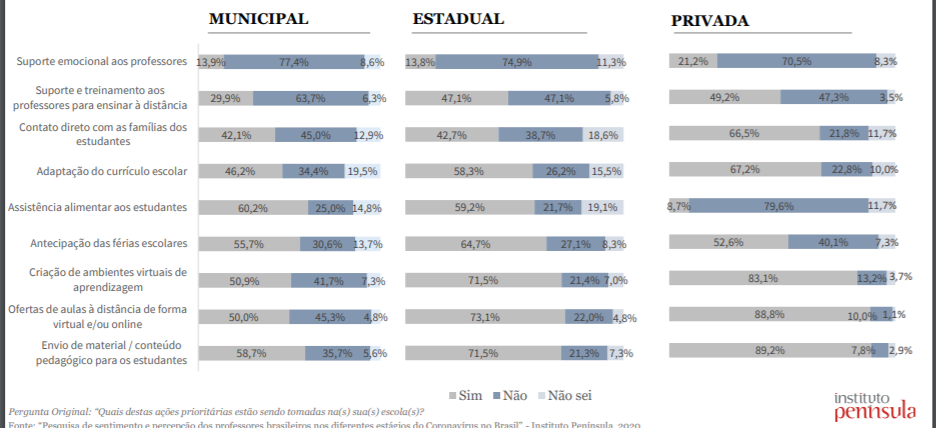
\includegraphics[width=0.90\textwidth]{Fig01}
 \caption{Quais ações as escolas têm realizado?}
 \label{Fig01}
 \source{Instituto Península.}
\end{figure}

Como é possível observar, de fato, é preciso mais assistência aos professores, tanto no quesito emocional quanto com relação ao seu desenvolvimento profissional, tendo em vista a escassez de assistência apresentada.

Em abril de 2020, o Programa Todos pela Educação lançou uma nota técnica sobre o Ensino a Distância na Educação Básica frente à pandemia da COVID-19\footnote{Nota técnica Ensino a distância na Educação Básica frente à pandemia da COVID-19. Disponível em: \url{https://www.todospelaeducacao.org.br/_uploads/_posts/425.pdf?1730332266=}. Acesso em: 30 maio, 2020.}, analisando a adoção de estratégias de ensino remoto diante do cenário de suspensão provisória de aulas presenciais. 

\begin{figure}[htbp]
 \centering
 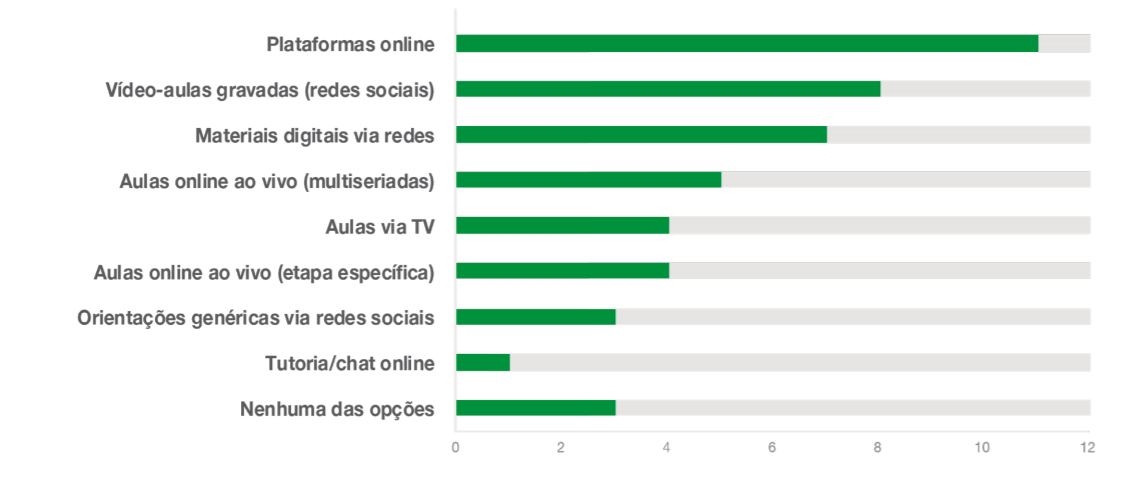
\includegraphics[width=0.90\textwidth]{Fig02}
 \caption{Estratégias das redes Estaduais.}
 \label{Fig02}
 \source{Todos Pela Educação.}
\end{figure}

\begin{figure}[htbp]
 \centering
 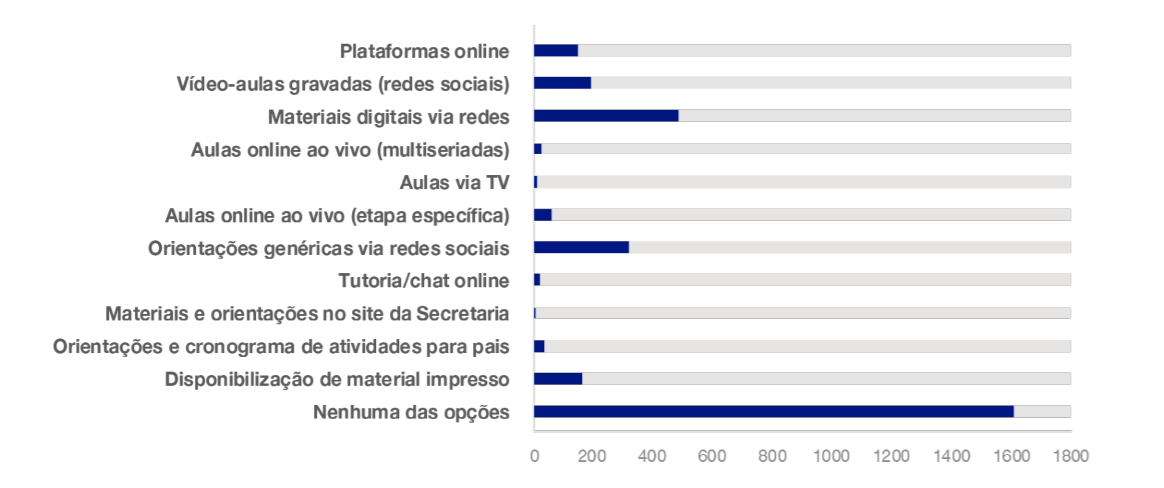
\includegraphics[width=0.90\textwidth]{Fig03}
 \caption{Estratégias das redes Municipais.}
 \label{Fig03}
 \source{Todos Pela Educação.}
\end{figure}

Nas \cref{Fig02} e \cref{Fig03}, observam-se estratégias das redes estaduais e municipais brasileiras de educação, respectivamente, realizadas no período da quarentena: usos de plataformas \textit{on-line}, gravação de videoaulas, disponibilização de materiais digitais via redes, aulas \textit{on-line} ao vivo (multisseriadas), aulas via TV, aulas \textit{on-line} ao vivo (etapa específica), orientações genéricas via redes sociais e tutoria/chat \textit{on-line}. As redes municipais, além dessas estratégias, ainda que em menor escala e proporção, também ofereceram materiais e orientações no site da Secretaria de Educação, orientações e cronograma de atividades para pais e disponibilização de material impresso. Apesar disso, o aumento de desigualdade em face dos alunos que não podem (ou não puderam) ter acesso a essas estratégias ou outras para continuarem os estudos de modo remoto tornou-se preocupante. 

Nesse sentido, \textcite{bunzen_o_2020} lança luzes para o fato de que há uma grande desigualdade econômica vivida por pessoas envolvidas no sistema educativo, que não possuem acesso à internet de qualidade ou ferramentas adequadas. Como destaca o autor, “Em muitas famílias, apenas um computador (de mesa ou portátil) ou um celular precisam ser compartilhados por vários usuários ao mesmo tempo” \cite[p. 24]{bunzen_o_2020}. Portanto, ao escolher ferramentas, plataformas e mídias, professores também precisam estar atentos a essas demandas.

Tais ações colocam em evidência – além de trabalhos ainda mais frequentes e consistentes nessa mesma direção – algumas necessidades, como a de adaptar e (re)editar planejamentos e as próprias aulas.

\section{Lições aprendidas e possíveis contribuições}\label{sec-licoes}
A COVID-19, com seus impactos\footnote{The impact of COVID-19 on education in Brazil. Disponível em: 
\url{https://www.worldbank.org/en/events/2020/04/29/the-impact-of-covid-19-on-education-in-brazil}. Acesso em: 30 maio, 2020.
Time to fix American education with race-for-space resolve. Acessado em: \url{https://news.harvard.edu/gazette/story/2020/04/the-pandemics-impact-on-education/}. Acesso em: 30 maio, 2020.
The Economic impact of the coronavirus pandemic. Acessado em: \url{https://www.washingtonpost.com/opinions/the-economic-impact-of-the-coronavirus-pandemic/2020/03/20/7e2e077a-6945-11ea-b199-3a9799c54512_story.html}. Acesso em: 30 maio, 2020.
Mental health and psychological resilience during the COVID-19 pandemic. Acessado em: \url{http://www.euro.who.int/en/health-topics/health-emergencies/coronavirus-covid-19/news/news/2020/3/mental-health-and-psychological-resilience-during-the-covid-19-pandemic}. Acesso em: 30 maio, 2020.}, trouxe desafios sem precedentes a toda a população mundial, mesmo àqueles que moram em lugares onde o vírus não chegou, pois, ainda que não estejam contaminados, podem assistir aos noticiários e perceber os números cada vez maiores, ter amigos e familiares em outros países e, assim, ser afetados de alguma forma pela doença.

\subsection{Os professores e as tecnologias digitais}\label{sec-professores}
Conforme os dados apresentados na seção anterior, para os professores, são significativos os desafios diante da crise atual. Principalmente, no que se refere a migrar para o ensino essencialmente mediado pelas tecnologias digitais. Estas têm sido, de fato, uma preocupação relevante em todo o cenário educacional brasileiro, no sentido de que é necessário aprender a usá-las de forma eficaz para ensinar. Ao utilizar os recursos e ferramentas tecnológicas diversas, é preciso ter em mente os alunos, suas necessidades e os objetivos, visando à sua aprendizagem.  

Com relação à adaptação ou à reedição das aulas, ações também necessárias para que o ensino funcione no novo formato imposto pela pandemia, \textcite{ribeiro_escrever_2018} destaca seis elementos, que apesar de serem relacionados ao uso de tecnologias, a autora entende ser de natureza humana e não material:

\textit{a) Vontade de aprender}

Para começar a usar tecnologias digitais novas em sala de aula, é preciso ter interesse e curiosidade de saber mais como elas funcionam, como usá-las, adaptá-las ou até melhorá-las. Ao utilizar uma plataforma de interação síncrona, como é o caso do Google Meets\footnote{Disponível em: \url{https://meet.google.com/}. Acesso em: 30 maio, 2020.} ou do Zoom\footnote{Disponível em: \url{https://zoom.us/}. Acessado em: 30 maio, 2020.}, por exemplo, há muito que aprender sobre cada uma, suas potencialidades, como elas podem intermediar o conhecimento, entre outros. O mesmo pode ser verdade sobre plataformas assíncronas. Assim, torna-se essencial experimentá-las e aprender como funcionam na prática.

\textit{b) Usar}

Para inserir uma ferramenta digital no planejamento, é preciso conhecer como ela funciona e usá-la em práticas sociais. Assim, professores poderão pensar em formas de adaptá-la para as aulas, tendo em mente os objetivos traçados previamente. Sem o uso pessoal, dificilmente será possível visualizar seus usos pedagógicos ou os problemas que poderão surgir. Por outro lado, apenas usar e não tornar viável o uso da ferramenta na atividade profissional faz com que os professores deixem de aproveitar o potencial que a tecnologia tem e pode acrescentar às suas práticas.

\textit{c) Relacionar}

Aqui, é importante que o professor, independentemente de sua idade ou do tempo de experiência que possua com o uso das tecnologias digitais, consiga relacionar o que planejou para a aula, considerando objetivos e/ou conteúdos, a uma nova forma de ensinar utilizando essas ferramentas. Deve-se pensar nas suas possibilidades, em como adaptar e levar algo novo para a sala de aula. Por isso, é relevante perguntar-se: o que planejei pode ser ensinado sem esses recursos e ferramentas? O que estou propondo vai ampliar as possibilidades de interação entre os alunos e deles comigo? Isso vai contribuir para que eles produzam mais e melhor? Poderei acompanhar melhor o processo de escrita, em tempo real ou por meio de registros? Se as repostas forem positivas, valerá a pena investir nos novos usos. 

\textit{d) Experimentar} 

Como saber se o que foi planejado pode dar certo? Experimentando. Será fundamental para o professor planejar a aula e pilotá-la, verificar se o dispositivo escolhido teve receptividade, quais foram os problemas apresentados, observar possíveis erros e acertos, para poder fazer os ajustes necessários, além de replicar e pensar em novas possibilidades para as aulas futuras.

\textit{e) Avaliar}

Nesse momento, a observação do uso é essencial. A ferramenta usada favoreceu a aprendizagem dos alunos ou não? O que foi adaptado, utilizado ocorreu como o planejado? Houve um envolvimento maior dos alunos? Facilitou meu trabalho? A avaliação da experiência servirá para “[...] ajustá-la, desistir ou avançar em outra proposta” \cite[p. 111]{ribeiro_escrever_2018}.

É importante destacar aqui que utilizar uma ferramenta nova não implica necessariamente o sucesso desse uso. Por isso é que se deve experimentá-la, vindo em seguida a reflexão sobre os resultados obtidos.  

\textit{f) Gestão do tempo de trabalho}

Nesses tempos em que as pessoas precisam trabalhar em casa (no formato \textit{home office}), é preciso delimitar o tempo de acompanhamento das atividades propostas \textit{on-line}. Com o uso de diferentes recursos e ferramentas tecnológicas, os professores ficam conectados por mais tempo na internet e isso faz com que tenham um aumento de demandas, inclusive com mensagens e cobranças de alunos e colegas fora de seu horário de trabalho. Por isso, deve-se aprender a gerir o tempo de atendimentos e atividades pedagógicas, investindo no planejamento e estabelecendo o equilíbrio e os devidos limites.

Independentemente de qual seja o plano de aprendizagem remota adotado ou as ferramentas escolhidas, é fato que é necessário que haja pertinência e relevância no contexto atual e para a vida dos alunos. Assim, não se pode apenas transpor o formato e o conteúdo de ensino presencial para as plataformas \textit{on-line}. É preciso pensar em novas formas de ensinar, considerar as novas maneiras de aprender e ressignificar, entre outros, o modo de avaliar. Isso poderá contribuir para que os próximos passos tomados sejam baseados nas necessidades observadas pelo professor em relação ao que os alunos precisam aprender, e como esse aprendizado poderá ocorrer. 

\subsection{As famílias e a reorganização das rotinas}\label{sec-familias}
Considerando também a educação e os novos arranjos na rotina familiar, observam-se depoimentos diversos em redes sociais que demonstram dificuldades na adaptação das famílias aos estudos dos filhos, tendo em vista que precisam conciliá-los não só com as tarefas domésticas, mas também com as atividades profissionais nessa nova realidade. 

Nessa perspectiva, realizou-se uma análise do discurso postado no Facebook, com base em elementos da Semiótica Francesa, ou Escola de Paris. De maneira breve, a proposta da Semiótica Francesa, que foi iniciada por \textcite{greimas_sobre_1975}, é dedicada ao estudo do conteúdo, assim como de sua arquitetura, considerando a maneira como o texto é organizado para expressá-lo. Além disso, ela valoriza o sentido na análise interna da produção textual, desde sua forma mais abstrata até certo grau de complexidade e concretude da mesma \cite{bertrand_caminhos_2003, brito__2012, pereira_o_2016}. 

\textcite[p. 2]{silva_avancos_2011} ressalta que a Semiótica Francesa é “[...] um ramo das ciências da linguagem que se ocupa dos conjuntos significantes”. Assim sendo, “[...] seu objeto de análise será sempre um signo, tomado no sentido amplo do termo (texto verbal, não verbal e sincrético), enfim, tudo que carreia um sentido”. Dessa forma, são analisados neste artigo textos de postagens, para compreender melhor o que dizem, atentando-se ao seu sentido, tendo em vista o contexto de ensino remoto.

Os depoimentos a seguir são comentários de mães de crianças em fase de alfabetização, retirados de páginas do Facebook no mês de abril de 2020, a respeito de suas vivências em casa, a partir da necessidade de ajudar os filhos com os estudos escolares de forma remota:

\begin{quote}
\textit{De boa... e a escola segue normal. A partir de segunda, o J. terá quatro aulas on line de matérias diversas. Decepção é o nome! Em que mundo esse pessoal vive? Nenhum pai trabalha em servico essencial ou não tem mais nada para fazer para fazer homeschooling ne} [S.V., Página no Facebook, 09/04/2020]

\textit{Segundo o plano da escola, como tenho 2, posso ficar dando aula para um a manhã toda, e a tarde para outro. Não preciso trabalhar e nem cuidar de nada da casa ... Sei... O pessoal aí deve ter empregada em casa, vive de renda e vai para a Disney em julho {\Symbola 😠} escola BOA antecipa férias!!@ e coitado dos professores que além do stress da quarentena além tem de dar aula on line [...] Eles acham. Que da para deixar uma. criança de 6 e 7 sozinhas para as aulas? Imagine! Fico do lado, eles se distraem e precisam de ajuda para fazer as atividades. Agora na cabeça do povo isso é aula normal}. [R.A., Página no Facebook, 09/04/2020]

\textit{E mãe trabalhando cheia de intimações... ANTECIPEM as férias!} [S.V., Página no Facebook, 17/04/2020]

\textit{Aqui é a mesma coisa...} [J.C., Página no Facebook, 17/04/2020]

\textit{Antecipem as FÉRIAS! Pelo amorrrrrr} [P.B., Página no Facebook, 17/04/2020]

\textit{E. não ficou nem 2 minutos [...] Férias já!!!!} [N.L., Página no Facebook, 17/04/2020]\footnote{Os nomes dos membros da rede social e das demais pessoas mencionadas nas postagens e comentários foram substituídos por abreviações, para preservar suas identidades.}
\end{quote}

%Nesta citação há emojis a adicionar

Nota-se que a mídia utilizada deu voz e cedeu espaço para desabafos de pessoas sobrecarregadas com a situação emergencial, que compartilham desde a dificuldade para ensinar os filhos em casa tendo que trabalhar, pedidos de antecipação das férias, até a capacidade de concentração das crianças. 

No nível do discurso, observa-se a tematização, que reflete sobre as “[...] formas de abordar/construir a realidade” \cite[p. 3]{brito__2012}, exemplificando e justificando o que está acontecendo no momento atual. A temática em torno da qual se desenvolve o discurso é a necessidade apresentada pelos participantes da conversa de as escolas decretarem férias, já que as famílias demonstram dificuldades para ensinar os filhos de forma remota e desempenhar seus papéis profissionais, ao mesmo tempo.

Observa-se também nos comentários a isotopia, um termo emprestado da Física. Na Semiótica, ela reitera a:

\begin{quote}
    [...] recorrência de traços semânticos que garantem a coerência de um texto (BARROS, 2001, p. 124). A isotopia é aquilo que assegura um plano de leitura (LARA; MATTE, 2009, p.70), o que não impede que ela seja quebrada em um dado texto ou que ela se oponha ou se alie à outra de modo que se produzam efeitos de sentido diversos: de crítica, de humor, de estranhamento etc. \cite[p. 3]{brito__2012}.
\end{quote}

Verifica-se que alguns trechos do texto apresentam teor crítico e, até mesmo, irônico: “Nenhum pai trabalha em servico essencial ou não tem mais nada para fazer para fazer homeschooling ne”, “Não preciso trabalhar e nem cuidar de nada da casa ... Sei...”, “O pessoal aí deve ter empregada em casa, vive de renda e vai para a Disney em julho”, “Agora na cabeça do povo isso é aula normal”.

\textcite[p. 131]{lemos_o_2014} destacam que as famílias da “era da informação” talvez estejam experimentando a era da “intercomunicação” e da “interconexão planetária” nas comunidades virtuais, que criam “[...] sociabilidade, redes de conversação e de ajuda mútua, a fim de revitalizar tanto as vizinhanças locais quanto os processos democráticos”. 

Conforme \textcite{boechat_as_2017}, a “era da informação” intensifica o uso das mídias digitais e o avanço das tecnologias tem incrementado seu desenvolvimento de forma acelerada. Pode-se dizer, então, que além de se apropriar melhor dessas mídias visando à continuação das atividades pedagógicas, é o momento para a escola desenvolver uma aproximação com as famílias de seus alunos por meio dessas ferramentas de comunicação e vice-versa. No entanto, será possível afirmar que tanto a escola quanto as famílias estão preparadas para lidar com toda a demanda que surgiu a partir da pandemia? 

Com isso, surge a necessidade de rever a velocidade com que os compromissos precisam ser cumpridos nos ambientes virtuais e a pressão social com a habilidade para usar as mídias digitais, cada vez mais presentes e que, com a pandemia, se intensificou entre as famílias e na escola. Essa “dromoaptidão” - a intimação da cultura para que os indivíduos sejam velozes quanto ao uso de apetrechos tecnológicos, a linguagem e os conhecimentos exigidos nesses meios, a capacidade para se atualizar com relação ao \textit{hardware}, \textit{software} e \textit{netware}, e o acesso à rede - pode segregar socialmente aqueles que não podem se apropriar da cultura digital \cite{boechat_as_2017}.
	
Assim, cabe, em tempos de crise como a que se discute aqui, priorizar a reorganização da rotina familiar para que o engajamento na educação dos filhos seja mais produtivo, estimulando a “inteligência coletiva”, que é entendida por \textcite{lemos_o_2014} como “potência de autocriação”, capacidade de “aprendizagem autônoma” e “processo de evolução”. Segundo os autores,

\begin{quote}
    [...] a propensão à inteligência coletiva representa o apetite para o aumento das capacidades cognitivas das pessoas e dos grupos, quer seja a memória, a percepção, as possibilidades de raciocínio, a aprendizagem ou a criação \cite[p. 14, grifos dos autores]{lemos_o_2014}.
\end{quote}

Portanto, a participação intencional na aprendizagem dos filhos, bem como o incentivo às suas inteligências coletivas podem contribuir para que eles tracem caminhos com maior protagonismo rumo à construção de seu próprio conhecimento.

\section{Considerações finais}\label{sec-organizacao}
As limitações da escola regular com relação ao mundo de hoje e de amanhã podem ser diversas, principalmente quando se trata de situações emergenciais, em que não há como ter controle nem mesmo do planejamento (o que em épocas “normais” já não é possível, tendo em vista que o professor constantemente precisa fazer ajustes e adaptações em seus planos de aula para atender a todos da melhor maneira possível), ou da situação vivida ao redor do mundo. É preciso, então, considerar cada escola com sua comunidade e sua realidade, para compreender o que acontece em seu contexto e poder sugerir-lhe medidas cabíveis e realizáveis.

A pandemia da COVID-19 trouxe desafios incontestáveis a todos. Com ela, surgiu a urgência de ressignificar os usos e também a pedagogia adotada pela escola e pelos professores, para que as práticas utilizadas anteriormente não sejam apenas reproduzidas nos ambientes virtuais durante as aulas remotas. 
	
Dessa forma, percebe-se que novos usos e novas perspectivas devem ser pensados, no sentido de aproximar ainda mais as famílias da escola e vice-versa. De fato, apesar da distância geográfica e temporal entre todos os envolvidos no ensino e na aprendizagem que se dão de modo virtual, não se pode negar que o recurso mais importante para que tudo aconteça não é a internet, nem os computadores ou as demais ferramentas utilizadas, mas os alunos e os professores, que fazem com que as experiências realizadas possam ser bem-sucedidas. 

Da mesma maneira, hoje, ainda mais do que antes, as famílias se tornaram peças-chave no processo de ensino e aprendizagem de seus filhos. Com uma crise instalada, tornou-se essencial, apesar de toda a dificuldade encontrada, ressignificar seu papel e acompanhar a educação dos filhos mais de perto, ensiná-los a gerir seu tempo de estudo e lazer, conciliar as atividades profissionais e domésticas para estarem disponíveis para ajudá-los com as tarefas escolares, aprender a utilizar as tecnologias digitais ou colocar em prática o que já sabiam nesse contexto. 

Enfim, tanto gestores como professores e famílias precisam ter a consciência de que o momento pandêmico é adverso e que é preciso haver cooperação entre todos, para que seja possível passar por ele aprendendo lições que serão valiosas no futuro. Portanto, estimular a inteligência coletiva das crianças e adolescentes pode significar o aumento de sua autonomia e protagonismo em sua própria aprendizagem na era da informação.

\printbibliography\label{sec-bib}

\end{document}
